\FloatBarrier
\section{Electrical Detection of Charge}
\label{app:charge-detection}

Sections~\ref{sec:electron-number-control}
and~\ref{sec:initialization-readout} use electrical signals to identify
changes in electron number and resolve the target charge. This appendix
derives the current through the target and the response of a separate
charge sensor.
\label{chap:experimental-measurement}

An electron entering or leaving a target dot can be observed in two
ways. If the target lies between a source and drain, repeated transfer
through it produces a current. If continuous transport is unavailable
or undesirable, a nearby sensor responds to the target occupation.
Both methods locate the same charge boundaries, but they record
different electrical signals.

\subsection{Current through a dot}
\label{sec:measurement-sequential-tunneling}

\subsubsection{Physical picture}
\label{sec:measurement-current-picture}

We seek the gate voltage $V_g$ at which the dot's equilibrium
electron number changes from $N-1$ to $N$. With all other electrode
voltages fixed, the addition energy is
$\mu_N(V_g)=E_N(V_g)-E_{N-1}(V_g)$, where $E_N$ is the
$N$-electron ground-state energy.

At zero temperature, a dot in equilibrium with a reservoir at
chemical potential $\mu_{\mathrm R}$ changes between $N-1$ and
$N$ electrons at
\begin{equation}
 \mu_N(V_g)=\mu_{\mathrm R}.
 \label{eq:measurement-transition-target}
\end{equation}
To locate this transition through a current, we couple the dot
to a source that supplies electrons and a drain that receives
them, with chemical potentials $\mu_{\mathrm S}>\mu_{\mathrm D}$
held fixed during each gate scan.
We treat tunneling as successive single-electron events and
neglect the energy width of the dot states caused by coupling to
the reservoirs. We choose the interval between the reservoir
chemical potentials narrow enough that only the $N-1\leftrightarrow N$
ground-state transition can enter it during this scan. For current
to flow, the source must have an occupied state at $\mu_N$, and
the drain an empty one. At zero temperature, the three regimes are
\begin{equation}
 \begin{aligned}
  \mu_{N-1}<\mu_{\mathrm D}<\mu_{\mathrm S}<\mu_N
   &:\quad \text{blocked at }N-1,\\
  \mu_{\mathrm D}<\mu_N<\mu_{\mathrm S}
   &:\quad \text{transport between }N-1\text{ and }N,\\
  \mu_N<\mu_{\mathrm D}<\mu_{\mathrm S}<\mu_{N+1}
   &:\quad \text{blocked at }N.
 \end{aligned}
 \label{eq:measurement-zero-temperature-window}
\end{equation}
The two fixed-charge regimes have zero sequential current and are
called \emph{Coulomb-blockade regions}.

The energy interval between $\mu_{\mathrm D}$ and $\mu_{\mathrm S}$
is called the \emph{bias window}. We control its width with the
source--drain bias $V_b$, defined by
\begin{equation}
 \mu_{\mathrm S}-\mu_{\mathrm D}=eV_b,\qquad e>0.
 \label{eq:measurement-bias-definition}
\end{equation}
The window has width $e|V_b|$; the sign of $V_b$ determines which
reservoir has the higher chemical potential. For negative bias,
interchange source and drain in
Eq.~\eqref{eq:measurement-zero-temperature-window}.
At positive bias with $\mu_N$ inside the window,
an electron tunnels from the source into the dot, changing its
electron number from $N-1$ to $N$. An electron then tunnels from
the dot into the drain, returning the dot to $N-1$ electrons.
Each cycle transfers one electron from source to drain, and
repeated cycles produce a steady current.

Our main scan varies $V_g$ to change the dot potential and hence
$\mu_N$, while the reservoir voltages keep the window fixed.
Between scans, we also adjust $V_b$ to select the window width. In
Figure~\ref{fig:transport-addition-window}, increasing $V_g$ lowers
$\mu_N$ through the window. The current turns on at
$\mu_N=\mu_{\mathrm S}$, when electron entry becomes possible,
and turns off at $\mu_N=\mu_{\mathrm D}$, when electron exit is
blocked. The measured current edges thus identify the gate
voltages that align $\mu_N$ with each reservoir. As the two
reservoir chemical potentials approach a common value
$\mu_{\mathrm R}$, these edges approach the equilibrium
transition voltage in
Eq.~\eqref{eq:measurement-transition-target}.

\begin{figure}[htbp]
 \centering
 % A rigid gate sweep through one isolated charge transition.
% All coordinates are schematic; the three settings are consistent
 % with the zero-temperature off--on--off current in the lower panel.
\begingroup
\definecolor{transportA}{HTML}{0072B2}
\definecolor{transportB}{HTML}{D55E00}
\definecolor{transportC}{HTML}{009E73}
% Logistic step, written using only nonpositive exponential arguments.
\pgfmathdeclarefunction{transportStep}{1}{%
 \pgfmathparse{0.5*(1+sign(#1)*(1-exp(-abs(#1)))/(1+exp(-abs(#1))))}%
}
\begin{tikzpicture}[
 x=1mm,y=1mm,>=stealth,line cap=round,line join=round,
 every node/.style={font=\small,inner sep=0pt}
]
 \path[use as bounding box] (0,8) rectangle (150,123);

 \begin{scope}
  \clip (17,56) rectangle (133,116);
  \fill[white] (17,56) rectangle (133,116);
  % The five thresholds have the same color at a given gate setting.
  \foreach \thresholdX/\thresholdY in {30/63,53/68,76/86,99/104,122/109}{
   \fill[transportA] (\thresholdX,{\thresholdY+6}) circle[radius=0.65mm];
   \fill[transportB] (\thresholdX,\thresholdY) circle[radius=0.65mm];
   \fill[transportC] (\thresholdX,{\thresholdY-6}) circle[radius=0.65mm];
  }
  % Real translucent masks are drawn AFTER the colored points.
  % The unmasked white strip is the window 83 < mu < 89.
  \fill[black!15,fill opacity=0.45,draw=none]
       (17,56) rectangle (133,83);
  \fill[black!15,fill opacity=0.45,draw=none]
       (17,89) rectangle (133,116);
 \end{scope}

 % Arrows between the target thresholds indicate increasing gate voltage.
 \draw[->,black!55,line width=0.45pt] (76,90.9)--(76,87.1);
 \draw[->,black!55,line width=0.45pt] (76,84.9)--(76,81.1);

 % No horizontal boundary strokes: shading alone delimits the window.
 \draw[->,line width=0.45pt] (17,56)--(136,56);
 \draw[->,line width=0.45pt] (17,56)--(17,119);
 \node[anchor=west] at (0,116) {(a)};
 \node[anchor=east] at (13,119) {$\mu_n$};
 \node[anchor=west] at (140,56) {$n$};
 \node[anchor=west] at (136,89) {$\mu_{\mathrm S}$};
 \node[anchor=west] at (136,83) {$\mu_{\mathrm D}$};
 \foreach \tickX/\tickLabel in {30/{N-2},53/{N-1},76/{N},99/{N+1},122/{N+2}}{
  \draw[line width=0.4pt] (\tickX,56)--(\tickX,54.8);
  \node at (\tickX,51.5) {$\tickLabel$};
 }

 % The plotted linear response is mu_N=86-3*(x-75)/17.
 % Thus mu_N crosses source 89 at x=58 and drain 83 at x=92.
 % The snapshots x=41,75,109 correspond to energy shifts +6,0,-6.
 \node[anchor=west] at (0,40) {(b)};
 \draw[->,black!70,line width=0.45pt] (17,13)--(136,13);
 \draw[->,black!70,line width=0.45pt] (17,13)--(17,42);
 \node[anchor=east] at (13,42) {$I$};
 \node[anchor=east] at (13,13) {$0$};
 \node[anchor=west] at (140,13) {$V_g$};
 \draw[black!85,line width=0.8pt]
      (21,13)--(58,13)--(58,35)--(92,35)--(92,13)--(131,13);
 % Finite-T current is the Fermi-function difference f_S-f_D.
 % In the rescaled gate coordinate, the thermal width is 1.7:
 % f_S-f_D = logistic((x-58)/1.7)-logistic((x-92)/1.7).
 % This is k_B T_e/(e V_b)=1.7/34=0.05, with the same unnormalized
 % current scale and tunnel rates as the zero-temperature trace.
 \draw[black!85,line width=0.85pt,dash pattern=on 2.3pt off 1.7pt]
      plot[domain=21:131,samples=221]
      (\x,{13+22*(transportStep((\x-58)/1.7)-transportStep((\x-92)/1.7))});
 \draw[black!85,line width=0.8pt] (105,39)--(113,39);
 \node[anchor=west] at (116,39) {$T_e=0$};
 \draw[black!85,line width=0.85pt,dash pattern=on 2.3pt off 1.7pt]
      (105,33)--(113,33);
 \node[anchor=west] at (116,33) {$T_e>0$};
\end{tikzpicture}
\endgroup

 \caption{Gate-controlled onset and suppression of transport.
 (a) Three colored sets of addition thresholds
 $\mu_n=E_n-E_{n-1}$ at increasing gate voltage; the arrows show
 their downward shift.
 The reservoir chemical potentials remain fixed. A translucent gray
 mask covers thresholds outside the narrow white zero-temperature
 bias window;
 only $\mu_N$ at the middle setting lies inside.
 (b) Current for the same bias and constant tunnel rates:
 zero temperature (solid) and finite temperature (dashed).
 The dashed curve follows
 Eq.~\eqref{eq:measurement-sequential-current}, with
 $k_BT_e/(\mu_{\mathrm S}-\mu_{\mathrm D})=0.05$.}
 \label{fig:transport-addition-window}
\end{figure}

Repeating the gate scan at different positive and negative biases
gives a two-dimensional current map $I(V_g,V_b)$. The Coulomb-blockade regions in
Eq.~\eqref{eq:measurement-zero-temperature-window} form
\emph{Coulomb diamonds} in this map
(Figure~\ref{fig:transport-coulomb-diamonds})~\cite{Beenakker1991}.

\begin{figure}[htbp]
 \centering
 % Schematic single-dot blockade map for locally linear gate response.
% Equal adjacent addition gaps and beta=1/2 give symmetric diamonds.
% Positive V_b means mu_S > mu_D, as in the chapter's convention.
\begingroup
\definecolor{diamondGate}{HTML}{0072B2}
\definecolor{diamondBias}{HTML}{D55E00}
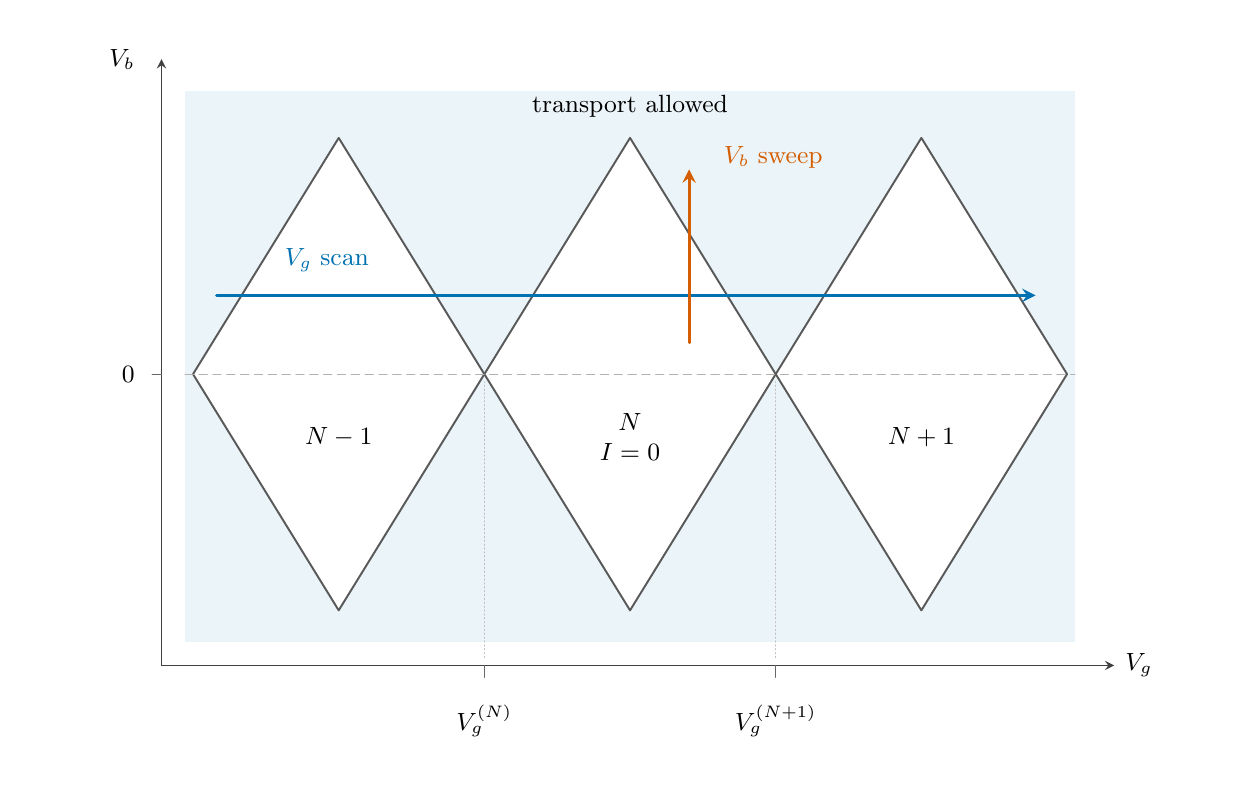
\begin{tikzpicture}[
 x=1mm,y=1mm,>=stealth,line cap=round,line join=round,
 every node/.style={font=\small,inner sep=1pt}
]
 \path[use as bounding box] (0,3) rectangle (150,96);

 % Pale regions admit charge transfer; white diamonds are blocked.
 \fill[diamondGate!8] (20,18) rectangle (133,88);
 \foreach \diamondLeft in {21,58,95}{
  \path[fill=white,draw=black!65,line width=0.7pt]
       (\diamondLeft,52)
       --({\diamondLeft+18.5},82)
       --({\diamondLeft+37},52)
       --({\diamondLeft+18.5},22)--cycle;
 }
 \draw[black!30,densely dashed,line width=0.4pt]
      (20,52)--(133,52);
 \node at (39.5,44) {$N-1$};
 \node[align=center] at (76.5,44) {$N$\\$I=0$};
 \node at (113.5,44) {$N+1$};

 % Two independent scan directions in voltage space.
 \draw[->,diamondGate,line width=1.1pt] (24,62)--(128,62);
 \node[text=diamondGate] at (38,66.5) {$V_g$ scan};
 \draw[->,diamondBias,line width=1.1pt] (84,56)--(84,78);
 \node[text=diamondBias,anchor=west] at (88,79.5) {$V_b$ sweep};
 \node at (76.5,86) {transport allowed};

 % Coordinate axes and zero-bias transition positions.
 \draw[->,black!75,line width=0.5pt] (17,15)--(138,15);
 \draw[->,black!75,line width=0.5pt] (17,15)--(17,92);
 \node[anchor=west] at (139,15) {$V_g$};
 \node[anchor=east] at (14,92) {$V_b$};
 \draw[black!60,line width=0.4pt] (15.8,52)--(17,52);
 \node[anchor=east] at (14,52) {$0$};
 \foreach \tickX in {58,95}{
  \draw[black!25,densely dotted,line width=0.4pt]
       (\tickX,16)--(\tickX,51);
  \draw[black!60,line width=0.4pt]
       (\tickX,15)--(\tickX,13.5);
 }
 \node at (58,8) {$V_g^{(N)}$};
 \node at (95,8) {$V_g^{(N+1)}$};
\end{tikzpicture}
\endgroup

 \caption{Gate and bias control of single-dot transport.
 White diamonds are fixed-charge regions with zero sequential
 current in the zero-temperature, negligible-broadening model.
 The surrounding tint marks energetically allowed transport,
 not the current magnitude. The blue horizontal arrow shows the
 main gate scan at fixed bias; the orange vertical arrow shows
 increasing positive bias at fixed gate voltage, widening the
 reservoir window. The voltages $V_g^{(N)}$ and $V_g^{(N+1)}$ are
 the zero-bias entry points of the $N$th and $(N+1)$th electrons.
 Equal diamond sizes and symmetric
 slopes are chosen for illustration; this is a schematic, not
 experimental data.}
 \label{fig:transport-coulomb-diamonds}
\end{figure}

\subsubsection{Deriving the current}
\label{sec:measurement-current-derivation}

We treat tunneling as successive, incoherent events between the
two charge states, keeping one nondegenerate ground state for each.
At zero temperature with $\mu_N$ inside the window, let
$\Gamma_{\mathrm S}$ and
$\Gamma_{\mathrm D}$ be the rates for entry from the source and
exit into the drain, in inverse seconds. Each rate is conditional
on the dot occupying the appropriate initial charge state;
Appendix~\ref{sec:amplitudes-to-master-equation} derives their
probability interpretation and the rate equation from quantum
transition amplitudes. If $p$ is the probability
that the dot contains $N$ electrons, then
\begin{equation}
 \dot p=\Gamma_{\mathrm S}(1-p)-\Gamma_{\mathrm D}p.
 \label{eq:measurement-zero-temperature-master-equation}
\end{equation}
The first term counts entries when the dot has $N-1$ electrons;
the second counts exits when it has $N$. This is the
\emph{sequential tunneling} description. Define $I$ as $e>0$ times the net electron-transfer
rate from source to drain; conventional electric current has the
opposite direction. In the stationary state, that transfer rate is
$\Gamma_{\mathrm D}p_{\mathrm{st}}$. Setting $\dot p=0$ therefore gives
\begin{equation}
 p_{\mathrm{st}}=\frac{\Gamma_{\mathrm S}}
                          {\Gamma_{\mathrm S}+\Gamma_{\mathrm D}},
 \qquad
 I=e\Gamma_{\mathrm D}p_{\mathrm{st}}
   =e\frac{\Gamma_{\mathrm S}\Gamma_{\mathrm D}}
             {\Gamma_{\mathrm S}+\Gamma_{\mathrm D}}.
 \label{eq:measurement-zero-temperature-current}
\end{equation}

With constant tunnel rates, this current is constant inside the
window and zero outside, giving the solid curve in
Figure~\ref{fig:transport-addition-window}(b).

At finite temperature, reservoir states near the chemical potential
are only partially occupied. Their occupation probability is the
Fermi function
\begin{equation}
 f_r(E)=\frac{1}{1+\exp[(E-\mu_r)/(k_BT_e)]},
 \qquad r=\mathrm S,\mathrm D,
 \label{eq:measurement-fermi-function}
\end{equation}
where $T_e$ is the reservoir electron temperature. To retain the
two-charge-state description, the excluded transitions must remain
outside the window by energy margins large compared with $k_BT_e$.
An entry event
requires an occupied reservoir state, whereas an exit event requires
an empty one. The rates become
\begin{equation}
 \Gamma_r^{\mathrm{in}}=\Gamma_r f_r(\mu_N),\qquad
 \Gamma_r^{\mathrm{out}}=\Gamma_r[1-f_r(\mu_N)].
 \label{eq:measurement-tunnel-rates}
\end{equation}
Here $\Gamma_r$ is the rate before the occupation factor is applied.
For a tunneling matrix element $v_r$ and a reservoir density of
states $\rho_r$ per unit energy, Fermi's golden rule gives
$\Gamma_r=2\pi|v_r|^2\rho_r/\hbar$. We treat these rates as nearly
constant across the transition. For the following finite-temperature
line shape, assume $\hbar(\Gamma_{\mathrm S}+\Gamma_{\mathrm D})
\ll k_BT_e$, so that thermal broadening dominates the level width
caused by tunneling, called \emph{lifetime broadening}. Spin or
orbital degeneracy is handled by including the corresponding states
and rates separately~\cite{Beenakker1991}.

Including entry and exit through both barriers generalizes the
zero-temperature rate equation to
\begin{equation}
 \dot p=(1-p)\sum_r\Gamma_r f_r(\mu_N)
        -p\sum_r\Gamma_r[1-f_r(\mu_N)].
 \label{eq:measurement-master-equation}
\end{equation}
Its stationary solution gives
\begin{equation}
 \begin{aligned}
 p_{\mathrm{st}}&=\frac{\Gamma_{\mathrm S}f_{\mathrm S}(\mu_N)
                  +\Gamma_{\mathrm D}f_{\mathrm D}(\mu_N)}
                         {\Gamma_{\mathrm S}+\Gamma_{\mathrm D}},\\
 I&=e\Gamma_{\mathrm S}[f_{\mathrm S}(\mu_N)-p_{\mathrm{st}}]
   =e\frac{\Gamma_{\mathrm S}\Gamma_{\mathrm D}}
             {\Gamma_{\mathrm S}+\Gamma_{\mathrm D}}
       [f_{\mathrm S}(\mu_N)-f_{\mathrm D}(\mu_N)].
 \end{aligned}
 \label{eq:measurement-sequential-current}
\end{equation}
Changing the bias changes the window and hence the current
through the factor
$f_{\mathrm S}(\mu_N)-f_{\mathrm D}(\mu_N)$.
Well inside the bias window, $f_{\mathrm S}(\mu_N)\simeq1$ and
$f_{\mathrm D}(\mu_N)\simeq0$, recovering
Eq.~\eqref{eq:measurement-zero-temperature-current}. Near either
edge, the gradual change in reservoir occupation rounds the
zero-temperature current step over an energy range of order $k_BT_e$,
as illustrated by the dashed curve in
Figure~\ref{fig:transport-addition-window}(b).

At zero bias, the two occupation factors are equal, so the net
current vanishes even at a charge transition. At finite temperature
and for $e|V_b|\ll k_BT_e$, the current is approximately linear in
bias: $I\simeq GV_b$, where $G=\partial I/\partial V_b|_{V_b=0}$
is the linear conductance. With a common equilibrium chemical
potential $\mu_{\mathrm R}$, expand the occupation
difference as $f_{\mathrm S}(\mu_N)-f_{\mathrm D}(\mu_N)
\simeq-eV_b f'(\mu_N)$, where $f$ is the common zero-bias
Fermi function. Substitution gives
\begin{equation}
 G=\frac{e^2}{4k_BT_e}
     \frac{\Gamma_{\mathrm S}\Gamma_{\mathrm D}}
          {\Gamma_{\mathrm S}+\Gamma_{\mathrm D}}
     \operatorname{sech}^2\!\left(
                  \frac{\mu_N-\mu_{\mathrm R}}{2k_BT_e}\right).
 \label{eq:measurement-conductance-peak}
\end{equation}
In this constant-rate model, the conductance peak is centered at
the gate voltage satisfying $\mu_N(V_g)=\mu_{\mathrm R}$.

\subsubsection{Experimental procedure}
\label{sec:measurement-current-procedure}

To perform the measurement, connect each reservoir through its
conducting contact to an external voltage output. Two outputs
sharing a reference conductor, called ground, can set the source
and drain voltages $V_{\mathrm S}$ and $V_{\mathrm D}$ independently.
The sign convention in Eq.~\eqref{eq:measurement-bias-definition}
corresponds to $V_b=V_{\mathrm D}-V_{\mathrm S}$.
One choice is $V_{\mathrm D}=0$ and $V_{\mathrm S}=-V_b$.
The electron path through the device is source--dot--drain, with a
tunnel barrier on either side of the dot
(Figure~\ref{fig:measurement-transport-path}). A separate voltage
output sets the gate voltage $V_g$ that changes the dot potential.

\begin{figure}[htbp]
 \centering
 % Transport panel extracted from measurement-paths.tex.
\begingroup
\small
\setlength{\unitlength}{1mm}
\linethickness{0.5pt}
\begin{picture}(150,37)
 \put(10,13){\framebox(34,15){\shortstack{source reservoir\\$\mu_{\mathrm S}$}}}
 \put(61,13){\framebox(28,15){target dot}}
 \put(106,13){\framebox(34,15){\shortstack{drain reservoir\\$\mu_{\mathrm D}$}}}
 \put(44,20.5){\vector(1,0){17}}
 \put(89,20.5){\vector(1,0){17}}
 \put(39,29){\makebox(72,5){electron transfer}}
 \put(10,3){\makebox(130,5){external circuit: bias source and current amplifier}}
\end{picture}
\endgroup

 \caption{Current through the target dot. Arrows indicate electron
 transfer from source to dot and from dot to drain. Reservoir
 contacts connect to an external circuit that sets their voltages
 and measures the current.}
 \label{fig:measurement-transport-path}
\end{figure}

A current amplifier in one external branch converts the current
into a voltage, $V_{\mathrm{out}}=R_{\mathrm{amp}}I$, where
$R_{\mathrm{amp}}$ is the measured gain in volts per ampere.
A digitizer samples this voltage, from which the current is
$I=V_{\mathrm{out}}/R_{\mathrm{amp}}$. A transfer rate of $10^6$
electrons per second gives only about $0.16$~pA, which sets the
scale of the required amplification.

Hold the reservoir voltages and barrier-gate settings fixed, and
step $V_g$ through the range of interest. After the current settles
at each point, store it together with $V_g$. At a bias for which
the current has a resolved plateau, its two edges give the gate
voltages satisfying $\mu_N=\mu_{\mathrm S}$ and
$\mu_N=\mu_{\mathrm D}$. In the linear regime
$e|V_b|\ll k_BT_e$, use $I/V_b$ to obtain the conductance and locate
its peak. The peak position gives the equilibrium transition
voltage in the small-bias limit.

To obtain the current map $I(V_g,V_b)$, repeat these gate scans
for a sequence of positive and negative biases. Keep the drain
voltage fixed and change the source voltage between scans to
adjust the window width and reverse the transport direction.

Keep the temperature low enough to resolve neighboring transitions,
and the tunnel rates sufficiently constant across the measured
feature for the derived current formulas to apply.
If the bias window admits another transition, reduce $|V_b|$ and
repeat the gate scan to recover an isolated transition before using
the two-charge-state current formula.

\subsubsection{Measuring the voltage response of an addition energy}
\label{sec:measurement-bias-spectroscopy}

A gate scan with a very small bias locates the conductance peak.
In the zero-bias limit, its position $V_g^0$ satisfies
$\mu_N(V_g^0,0)=\mu_{\mathrm R}$, as in
Eq.~\eqref{eq:measurement-conductance-peak}. This determines the
addition energy at one voltage setting. We now want to determine
how $\mu_N$ changes with gate voltage $V_g$ and bias $V_b$.

Keep the drain voltage fixed and vary the source voltage, so that
$\mu_{\mathrm D}=\mu_{\mathrm R}$ and
$\mu_{\mathrm S}=\mu_{\mathrm R}+eV_b$. Choosing the fixed
$\mu_{\mathrm R}$ as the energy zero, a first-order expansion
about $(V_g^0,0)$ gives
\begin{equation}
 \mu_N(V_g,V_b)\simeq-e\alpha(V_g-V_g^0)+e\beta V_b.
 \label{eq:measurement-biased-level}
\end{equation}
Here $\alpha=-(1/e)\partial\mu_N/\partial V_g$ and
$\beta=(1/e)\partial\mu_N/\partial V_b$ are evaluated at
$(V_g^0,0)$, with the other electrode settings fixed.

To measure these coefficients, widen the window enough to resolve
its two current edges, while keeping the transition isolated.
Repeat the gate scan at several nearby positive biases and record
the gate voltages at both edges. The two edges satisfy
$\mu_N=\mu_{\mathrm D}=0$ and $\mu_N=\mu_{\mathrm S}=eV_b$.
Substituting these two conditions into
Eq.~\eqref{eq:measurement-biased-level} gives the local edge lines
\begin{equation}
 V_b=\frac{\alpha}{\beta}(V_g-V_g^0),\qquad
 V_b=-\frac{\alpha}{1-\beta}(V_g-V_g^0).
 \label{eq:measurement-diamond-slopes}
\end{equation}
Fit these edges in the $(V_g,V_b)$ map, with bias on the vertical
axis. For $\alpha>0$ and $0<\beta<1$, their slopes are
$m_+>0$ and $m_-<0$. Solving for the two coefficients gives
\begin{equation}
 \alpha=\frac{m_+|m_-|}{m_++|m_-|},\qquad
 \beta=\frac{|m_-|}{m_++|m_-|}.
 \label{eq:measurement-lever-arm-calibration}
\end{equation}
The scan thus determines the desired local responses
$\partial\mu_N/\partial V_g=-e\alpha$ and
$\partial\mu_N/\partial V_b=e\beta$.

As an additional use, $\alpha$ converts the separation of adjacent
conductance peaks into an estimate of the addition-energy spacing.
Let their zero-bias positions be $V_g^{(N)}$ and $V_g^{(N+1)}$,
with $\Delta V_g=V_g^{(N+1)}-V_g^{(N)}$. If both thresholds shift
approximately with a common response $-e\alpha$ over this interval,
then their energy difference at the same gate voltage is
\[
 E_{\mathrm{add}}(N)
 =\mu_{N+1}(V_g,0)-\mu_N(V_g,0)
 \simeq e\alpha\Delta V_g.
\]
For this estimate, use a representative $\alpha$ measured near
the two peaks.

\subsection{A separate charge sensor}
\label{sec:measurement-charge-sensor}

We want to determine the target dot's electron number even when
electron transfer through it is too slow to give a measurable
steady current. A nearby detector can instead sense the electric
field of the target charge. The measured current passes through
the detector, so a charge change in the target can be detected
without repeated electron transfer through the target.
The sensor can also distinguish target charge configurations after
the target's reservoir barrier has been closed, because their
electric interaction with the sensor remains.

For a concrete setup, let the target exchange electrons with one
reservoir at chemical potential $\mu_{\mathrm R}$. This reservoir
can supply or accept an electron as the target gate voltage $V_g$
is varied. At low temperature, the equilibrium electron number
minimizes $E_N(V_g)-\mu_{\mathrm R}N$, with all other electrode
voltages fixed. A boundary between neighboring charge states
therefore occurs at $\mu_N(V_g)=E_N(V_g)-E_{N-1}(V_g)=\mu_{\mathrm R}$.
Holding the reservoir contact voltage fixed keeps $\mu_{\mathrm R}$
fixed; scanning $V_g$ changes the target potential and hence
$\mu_N$. We seek the gate voltage at which the electron number
changes, using the detector signal to identify that change.

We model the detector as a second dot connected to its own source
and drain, using the sequential-tunneling description of
Section~\ref{sec:measurement-sequential-tunneling}. Its steady
current $I_{\mathrm s}(\mu_{\mathrm s})$ follows
Eq.~\eqref{eq:measurement-sequential-current}, with $\mu_N$ replaced
by the sensor's addition energy $\mu_{\mathrm s}$ and with the
Fermi functions and tunnel rates taken for the sensor's own
reservoirs. With these reservoir voltages and tunnel rates held
fixed, a change in the target charge shifts $\mu_{\mathrm s}$
through the electric interaction between the dots and thereby
changes $I_{\mathrm s}$. This is \emph{charge sensing}.

For a simple density interaction
$H_{\mathrm{int}}=U_{\mathrm{sd}}\widehat N\widehat n_{\mathrm s}$,
$\widehat N$ counts target electrons, $\widehat n_{\mathrm s}$ counts
sensor electrons, and $U_{\mathrm{sd}}$ is an interaction energy.
Adding one sensor electron increases this interaction energy by
$U_{\mathrm{sd}}N$, so the same quantity contributes to the sensor's
addition energy. A change $\delta N$ in the target electron number
shifts the sensor addition energy by
$\delta\mu_{\mathrm s}=U_{\mathrm{sd}}\,\delta N$.
This shift moves the sensor threshold relative to the fixed source
and drain chemical potentials, changing the availability of
tunneling through the sensor.
For a small shift about the chosen sensor setting, the current
change is
\begin{equation}
 \delta I_{\mathrm s}\simeq
   \frac{\partial I_{\mathrm s}}{\partial\mu_{\mathrm s}}
      U_{\mathrm{sd}}\,\delta N.
 \label{eq:measurement-sensor-transduction}
\end{equation}
We therefore choose a sensor setting on a sloping part of its
independently measured current curve, where
$\partial I_{\mathrm s}/\partial\mu_{\mathrm s}$ is appreciable.
For a larger shift, the two current levels are calibrated directly.
A narrow conducting constriction, called a \emph{quantum point
contact}, can play the same role: target charge changes its barrier
and hence its transmission.

For two target dots, let $U_{\mathrm{s}1}$ and $U_{\mathrm{s}2}$
be their respective interaction energies with the sensor. The
sensor addition energy then changes by
\begin{equation}
 \delta\mu_{\mathrm s}
   =U_{\mathrm{s}1}\delta N_1+U_{\mathrm{s}2}\delta N_2.
 \label{eq:measurement-sensor-charge-configuration}
\end{equation}
A transfer $(1,1)\to(0,2)$ has $\delta N_1=-1$ and $\delta N_2=+1$.
It therefore shifts the sensor threshold by
$U_{\mathrm{s}2}-U_{\mathrm{s}1}$ even though the total target
electron number is unchanged. Distinguishing these configurations
requires different sensitivity to charge on the two dots; equal
couplings would give no signal for the transfer in this model.
This spatial sensitivity is needed for the singlet--triplet
readout in Section~\ref{sec:pauli-blockade-readout}.

For several target dots, a local model of the recorded sensor
signal is
\begin{equation}
 s(t)=s_{\mathrm{bg}}(\mathbf V)
         +\sum_i\kappa_i N_i(t)+\xi(t).
 \label{eq:measurement-sensor-signal}
\end{equation}
Here $s$ may be a sensor current or an amplified voltage,
$s_{\mathrm{bg}}$ is the response at fixed target charge to the
applied gate voltages $\mathbf V$, $\kappa_i$ is the signal change
per electron on dot $i$, and $\xi$ is detector noise. This expression
assumes approximately constant sensitivity over the small range
being measured. It is a model for the signal conditioned on a charge
record; averaging many records replaces $N_i(t)$ by
$\langle\widehat N_i(t)\rangle$.

A tunnel event produces a step between sensor levels. Monitoring
these steps reveals loading and unloading even when the target
has only one reservoir, so no source--drain path exists through it.
If the detector resolves individual events, this is a time-resolved
charge measurement~\cite{Thalakulam2011}.
In particular, an electron leaving a dot and a subsequent loading
event produce two steps that delimit a temporarily empty interval.
Sensor noise limits the distinction between current levels, and
a finite response time can hide an empty interval that is too short.

In the experiment, first scan the sensor gate to find a conductance
peak, then set the sensor on its side, where
$\partial I_{\mathrm s}/\partial\mu_{\mathrm s}$ is large. Establish
the two sensor signal levels corresponding to neighboring target
charge states. Hold the target reservoir voltage fixed and scan
the target plunger gate, allowing time for electron exchange with
the reservoir at each setting. A step between the calibrated levels
marks loading or unloading. If the scan also shifts the sensor
directly, compensate with its gate or measure and subtract the
smooth background $s_{\mathrm{bg}}$.

For a time-resolved record, keep the target settings fixed near a
loading or unloading condition and record the sensor signal as a
function of time. Individual steps then give event times.
Figure~\ref{fig:measurement-sensor-path} shows the connections for
a sensor coupled to two target dots.

\begin{figure}[htbp]
 \centering
 % Sensor panel extracted from measurement-paths.tex.
\begingroup
\small
\setlength{\unitlength}{1mm}
\linethickness{0.5pt}
\begin{picture}(150,38)
 \put(10,25){\framebox(34,11){target reservoir}}
 \put(61,25){\framebox(28,11){target dot 1}}
 \put(106,25){\framebox(34,11){target dot 2}}
 \put(44,30.5){\vector(1,0){17}}
 \put(89,30.5){\vector(1,0){17}}
 \put(75,11){\multiput(0,0)(0,2.3){6}{\line(0,1){1.2}}}
 \qbezier[18](123,25)(103,18)(83,11)
 \put(7,13){\makebox(60,8){electrostatic interaction}}
 \put(10,0){\framebox(34,11){sensor source}}
 \put(61,0){\framebox(28,11){sensor dot}}
 \put(106,0){\framebox(34,11){sensor drain}}
 \put(44,5.5){\vector(1,0){17}}
 \put(89,5.5){\vector(1,0){17}}
\end{picture}
\endgroup

 \caption{Charge detection with a separate sensor. Current passes
 through the sensor dot. The target charges change its addition
 threshold through the electric interaction between the dots.
 Horizontal arrows indicate tunnel connections; broken lines
 indicate electric interactions.}
 \label{fig:measurement-sensor-path}
\end{figure}
